\chapter{Internet Management}

\section{Overview}

Per gestire una rete, il suo traffico o la sua sicurezza è necessario prima di tutto che la rete funzioni.\
È quindi necessario un \textbf{metodo di comunicazione fra componenti di rete} per sapere se va tutto bene oppure no.\

\begin{table}[H]
    \centering
    \begin{tabular}{l l l}
        1987 & Simple Gateway Monitoring Protocol (SGMP)  &                 \\
        1987 & High-level Entity Management System (HEMS) &                 \\
        1988 & Simple Network Management Protocol         & proposed        \\
        1990 & Simple Network Management Protocol         & standard 15, 16 \\
        1991 & Management Information Base II             & standard 17     \\
        1993 & SNMP Version 2 (Party/Party/Context)       & historical      \\
        1996 & SNMP Version 2 (Communities)               & draft           \\
        1998 & SNMP Version 3 (User-based)                & draft           \\
    \end{tabular}
\end{table}

\noindent Quando furono creati i primi protocolli per la \textbf{gestione di Internet} vennero prese le idee base di ICMP:\ creare un \textbf{set d'istruzioni minimo per capire se la rete stesse funzionando ed in caso negativo cosa stesse andando male}.\
La caratteristica fondamentale di SNMP è l'essere \textbf{semplice}.\
Tale semplicità ha permesso il supporto del protocollo su apparecchi di rete con un costo ragionevole:\ ``\textit{gli switch di fascia medio-bassa possono essere gestiti tutti con SNMP}''.

SNMPv1 ha una grande diffusione soprattutto nella comunicazione dei dati.\
I tentativi di standardizzazione di SNMPv2 sono falliti.\
SNMPv3 con SNMPv1 è stato accettato da un'ampia comunità di produttori di reti.\
La comunità degli utenti ha accettato molto bene SNMPv3 in termini di supporto e sviluppo.

\subsubsection{SNMP Development Goals}

\begin{itemize}
    \item Minimizzazione del numero e della complessità delle funzioni di gestione che sono implementate da un agente:\
          \begin{itemize}
              \item Riduzione dei costi di sviluppo per agenti gestionali (applicazioni semplici).
              \item Ubiquity:\ utilizza la stessa tecnologia di gestione per tutti i dispositivi (stampanti o Cray).
              \item Estendibilità dell'applicazione:\ sviluppo di nuove funzioni di gestione senza la necessità di modificare gli agenti.
          \end{itemize}
    \item Estensibilità definendo nuovi MIB.
    \item Indipendenza da architetture di computer o di rete esistenti.
    \item Robustezza grazie a un semplice servizio di trasporto senza connessione (UDP).%attacchi DoS: in un server con un massimo di 10 connessioni, posso occupare tutte le connessioni e stare in silenzion
    \item Nessuna dipendenza da altri servizi di rete.
    \item L'aggiunta della gestione a dispositivi{\slash}applicazioni nuovi{\slash}esistenti dovrebbe essere poco costosa, semplice da sviluppare e con funzionalità limitate.
\end{itemize}
Purtroppo alcuni di questi obiettivi originari sono andati persi:\ il termine ``semplice'' si riferisce al protocollo e non alle specifiche o all'implementazione di applicazioni gestionali.

\subsubsection{Trap Directed Polling}

Il manager \textbf{esercita il controllo} su vari Agent eseguendo richieste continue (\textbf{polling}):\ poiché viene usato UDP per mandare messaggi, non è possibile conoscere gli stati degli Agent in ogni momento e quindi è necessario richiederli periodicamente; usando TCP ciò non sarebbe necessario perché la connessione persistente sarebbe sufficiente per conoscere lo stato dell'agente.\

Si ipotizzi che l'intervallo di tempo che passa fra un poll ed un altro sia di cinque minuti:\ \textbf{il Manager è cieco nei confronti dell'Agent a intervalli di cinque minuti}, ovvero assume che l'agent rimanga attivo/nello stesso stato per i cinque minuti successivi alla risposta.\
Questo non è sempre vero:\ l'Agent potrebbe ``rompersi'' subito dopo aver risposto al poll.\

Per risolvere questo problema gli Agent effettuano \textbf{trap} al Manager informandolo quando avviene un \textbf{cambio di stato importante}.\
Tuttavia l'Agent è in grado di \textbf{effettuare una trap se l'evento non è catastrofico} perciò il polling periodico è comunque necessario.\
Questo periodo di tempo varia a seconda dell'affidabilità dell'Agent con cui il Manager ha a che fare:\ \textbf{un Manager scritto bene riporta un concetto di fiducia} al suo interno, ovvero tenderà ad effettuare polling più spesso verso quegli Agent che si sono dimostrati meno affidabili.

In sintesi, i managers SNMP interrogano a intervalli regolari gli agenti SNMP:\ gli agents possono segnalare casi eccezionali a un manager inviando una trap; il manager SNMP può adattare la strategia di polling alla ricezione di trap (polling diretto da trap).

\begin{figure}[H]
    \centering
    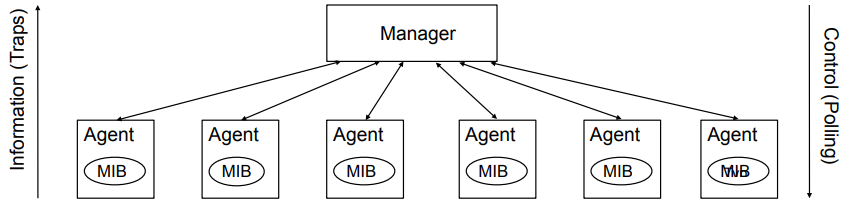
\includegraphics[width=\textwidth]{immagini/Trap_direct_polling.png}
\end{figure}

\noindent SNMP è un modello rigorosamente centralizzato, in cui il manager implementa l'intera funzionalità e responsabilità.

\subsubsection{SNMP Application Areas}

SNMP non è utilizzato solo per la gestione della rete, ma anche per il controllo e monitoraggio dei processi produttivi e dei sistemi informatici complessi e per il monitoraggio di programmi applicativi complessi (database relazionali, componenti SAP R{\slash}3,\ \dots).\

Sul mercato sono disponibili molti toolkit SNMP buoni, ma sono disponibili pochissime applicazioni per risolvere problemi di gestione complessi:\ l'implementazione di applicazioni speciali, o la conversione delle linee guida della procedura locale, in genere è relativamente complessa e costosa.

\section{Structure of Management Information \- (SMIv2)}

L'attuale modello di informazioni noto come ``\textit{Structure of Management Information version} 2'' (SMIv2) è definito e si basa su semplici variabili tipizzate, in particolar modo si basa sul sottoinsieme esteso di ASN.1 (1998).\
Ogni variabile ha un tipo di dati ASN.1 primitivo, non assemblato:
\begin{itemize}
    \item \texttt{INTEGER}, \texttt{OCTET STRING}, \texttt{OBJECT IDENTIFIER}, \texttt{NULL}
    \item \texttt{Integer32}, \texttt{Unsigned32}, \texttt{Gauge32}, \texttt{Counter32}, \texttt{Counter64}, \texttt{Ip\-Ad\-dress}, \texttt{TimeTicks}, \texttt{Opaque}
\end{itemize}
Non implementa strutture dati complesse e operazioni sulle variabili.\

Le variabili sono \textbf{scalari} (esattamente un'istanza) o colonne in una \textbf{tabella} bidimensionale ``concettuale'' (zero o più variabili) e su di esse possono essere applicate solo le operazioni di ``read'' e ``write''.\ Tuttavia il protocollo SNMP consente la manipolazione di elenchi di variabili.

I MIB (Management Information Bases) SMIv2 vengono definiti utilizzando speciali macro ASN.1.\
Sfrutta la complessità delle nuove definizioni di MIB:\ definizione di funzionalità di base e di tipi primitivi da utilizzare nei nuovi MIB.

\begin{figure}[H]
    \centering
    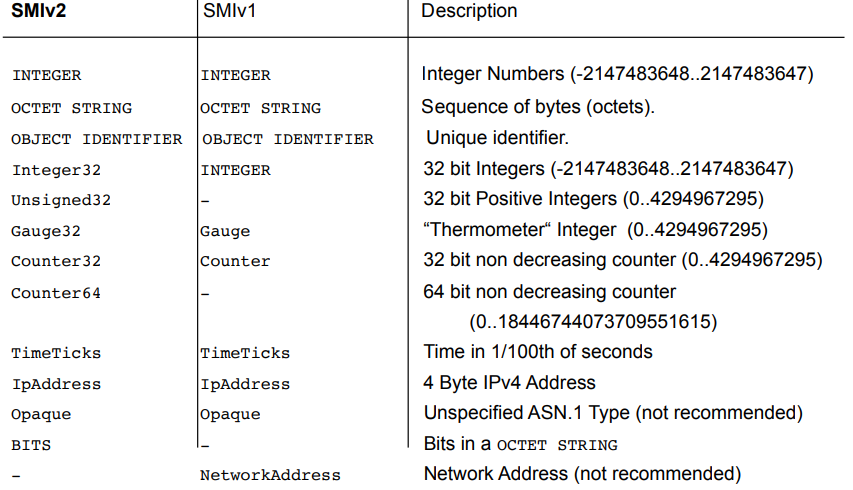
\includegraphics[width=\textwidth]{immagini/SMIv2_Basic_Datatypes.png}
    \caption*{SMIv2 Basic Datatypes (RFC 2578)}
\end{figure}

\noindent Un'altra caratteristica di SMI è che il tipo intero non si usa moltissimo, si preferisce utilizzare \texttt{gouge} e \texttt{counter}:\ sono entrambi interi ma possiedono una semantica ben precisa.\
Un \texttt{gouge} è un numero che rappresenta una quantità che va da un minimo ad un massimo.\
La temperatura, ad esempio, è un gouge (non bisogna farci calcoli sopra e può aumentare rimanendo tra un minimo ed un massimo, quando lo si legge quindi si estrapola il valore definitivo).\
Un \texttt{counter} è un intero a 32 bit come \texttt{gouge}, ma ha delle proprietà diverse:\ il contatore, infatti, non decresce (o rimane del valore corrente o aumenta) e il valore estrapolato da una variabile con questo tipo non è utilizzabile nell'immediato, ma lo si può usare per differenza (tachimetro dell'automobile e voglio sapere in un giorno quanti chilometri ho fatto).

\subsubsection{A MIB Use Case}

\begin{figure}[H]
    \centering
    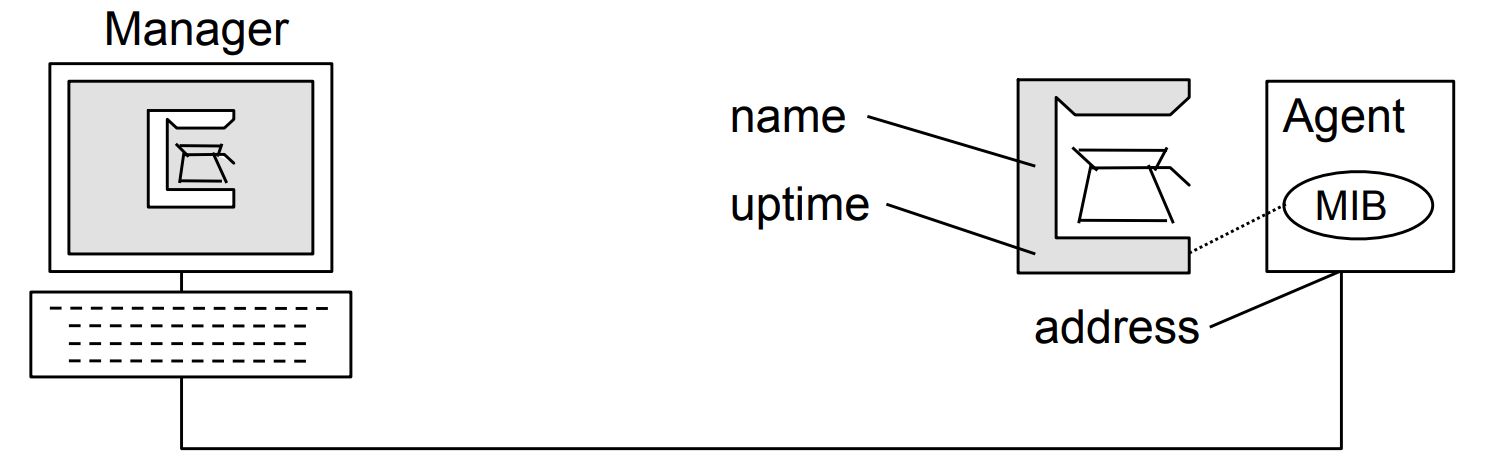
\includegraphics[width=0.8\textwidth]{immagini/MIB_useCase.png}
\end{figure}

Definizione delle variabili nell'ISO Registration tree.\
I nodi vengono definiti a scopo di denominazione.\
Le foglie dell'albero rappresentano gli oggetti gestiti (cioè ``la carne'').\
I nodi secondari possono essere utilizzati per organizzare logicamente i tipi di oggetto.\

\begin{figure}[H]
    \centering
    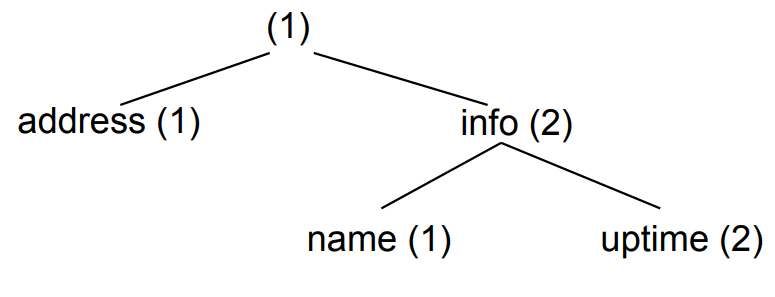
\includegraphics[width=0.5\textwidth]{immagini/ISO_registration_tree.png}
\end{figure}

\subsection{Object Identifier and Instance Identifier}

Nel Registration tree ogni oggetto può essere identificato mediante un object identifier univoco.\
Gli sviluppi concreti (istanza) di un tipo di oggetto sono designati univocamente da un cosiddetto \textit{identificatore di istanza}.\
Un identificatore di istanza univoco si ottiene allegando identificatori di istanza all'identificatore di oggetto.

Gli oggetti scalari hanno fondamentalmente \textbf{una sola istanza} il cui identificatore ha valore 0 (e.g.\ \texttt{sysName.0}).\
Gli identificatori di istanza per le variabili non scalari derivano dalla denominazione univoca di una tabella concettuale.\
Poiché l'identificatore di oggetto può contenere fino a 128 elementi, i nomi delle istanze non possono essere infinitamente complessi.
\begin{figure}[H]
    \centering
    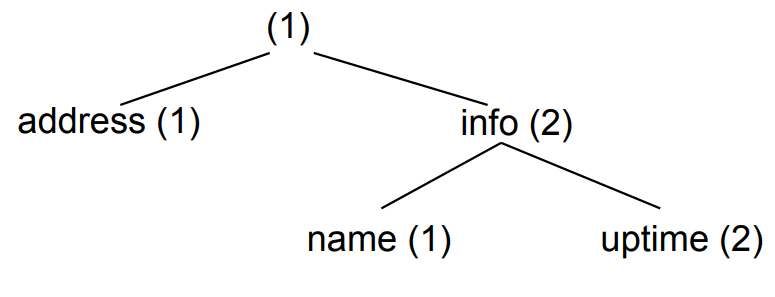
\includegraphics[width=0.5\textwidth]{immagini/ISO_registration_tree.png}
\end{figure}
\begin{table}[H]
    \centering
    \begin{tabular}{|l l l l|}
        \hline
        Object Identifier & Instance Identifier & Type                  & Value           \\\hline
        1.1               & 0                   & \texttt{IpAddress}    & 10.1.2.1        \\
        1.2.1             & 0                   & \texttt{OCTET STRING} & ``FilterFresh'' \\
        1.2.2             & 0                   & \texttt{TimeTicks}    & 54321           \\\hline
    \end{tabular}
\end{table}

\noindent I nomi dei nodi MIB sono rilevanti solo per gli utenti umani.

I descrittori devono essere univoci all'interno di un modulo MIB, sebbene possano essere utilizzati più volte in diversi moduli MIB (si ottengono descrittori univoci dalla combinazione dei nomi dei moduli e dei descrittori).

\begin{figure}[H]
    \centering
    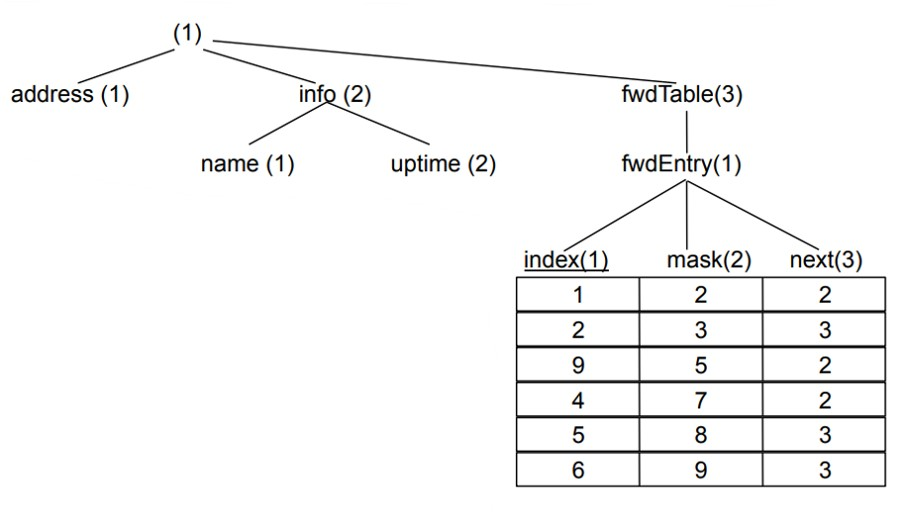
\includegraphics[width=0.7\textwidth]{immagini/Tables_MIB.jpg}
\end{figure}

\noindent Le tabelle sono definite fondamentalmente con due ``nodi ausiliari'':\ il primo nodo definisce la tabella ed è di tipo \texttt{SEQUENCE OF}, mentre il secondo nodo definisce una voce (una riga) nella tabella ed è di tipo \texttt{SEQUENCE}; questo è l'unico uso consentito di \texttt{SEQUENCE} e \texttt{SEQUENCE OF} in SNMP SMIv2.\

Il risultato della colonna e dell'identificatore di istanza (codice della tabella) è un identificatore di oggetto univoco per ciascuna voce di tabella.

\begin{table}[H]
    \centering
    \begin{tabular}{|l l l|l l l|l l l|}
        \multicolumn{9}{c}{Esempio di tabella (convenzione OID $\Rightarrow$ valore):}                          \\\hline
        1.3.1.1.1 & $\Rightarrow$ & 1 & 1.3.1.3.1 & $\Rightarrow$ & 2 & 1.3.1.2.4 & $\Rightarrow$ & 7           \\
        1.3.1.2.1 & $\Rightarrow$ & 2 & 1.3.1.1.4 & $\Rightarrow$ & 4 & 1.3.1.2.7 & $\Rightarrow$ & inesistente \\\hline
    \end{tabular}
\end{table}

\subsubsection{Tables Naming}

La denominazione delle tabelle è molto importante poiché influisce sul modo in cui si accede alle tabelle stesse.\
Ne esistono due tipi:\ uno usa numeri di riga (non utilizzati da SNMP), l'altro usa una colonna indice (il metodo usato da SNMP).

Un indice di tabella non è necessariamente un \texttt{INTEGER}, ad esempio la routing table utilizza un indirizzo IP come indice della tabella.

\begin{table}[H]
    \centering
    \begin{tabular}{|l|c|l|}
        \hline
        \multicolumn{3}{|c|}{Routing Table}                                   \\\hline\hline
        \texttt{destination}(1) & \texttt{policy}(2) & \texttt{next}(3)       \\\hline
        \texttt{130.89.16.23}   & 1                  & \texttt{130.89.16.23}  \\
        \texttt{130.89.16.23}   & 2                  & \texttt{130.89.16.127} \\
        \texttt{192.168.10.12}  & 1                  & \texttt{172.16.1.18}   \\
        \texttt{192.168.10.12}  & 2                  & \texttt{172.16.1.12}   \\\hline
    \end{tabular}
\end{table}

\noindent Un indice di tabella può essere composto da più componenti:

\begin{center}
    X .\ C .\ I\textsubscript{1} .\ I\textsubscript{2} \dots\dots\ I\textsubscript{n}
\end{center}

\begin{table}[H]
    \centering
    \begin{tabular}{c l}
        X                   & OID of the table:\ identifica la tabella \\
        C                   & Column number:\ identifica la colonna    \\
        $\rm I_1 \dots I_n$ & Index value (indice nella colonna)       \\
    \end{tabular}
\end{table}

\noindent Una tabella di routing IP è la combinazione di indirizzo IP e maschera di rete IP necessaria per soddisfare le regole di instradamento.\
I singoli byte dell'indirizzo IP vengono specificati come identificatori secondari individuali.

\begin{figure}[H]
    \centering
    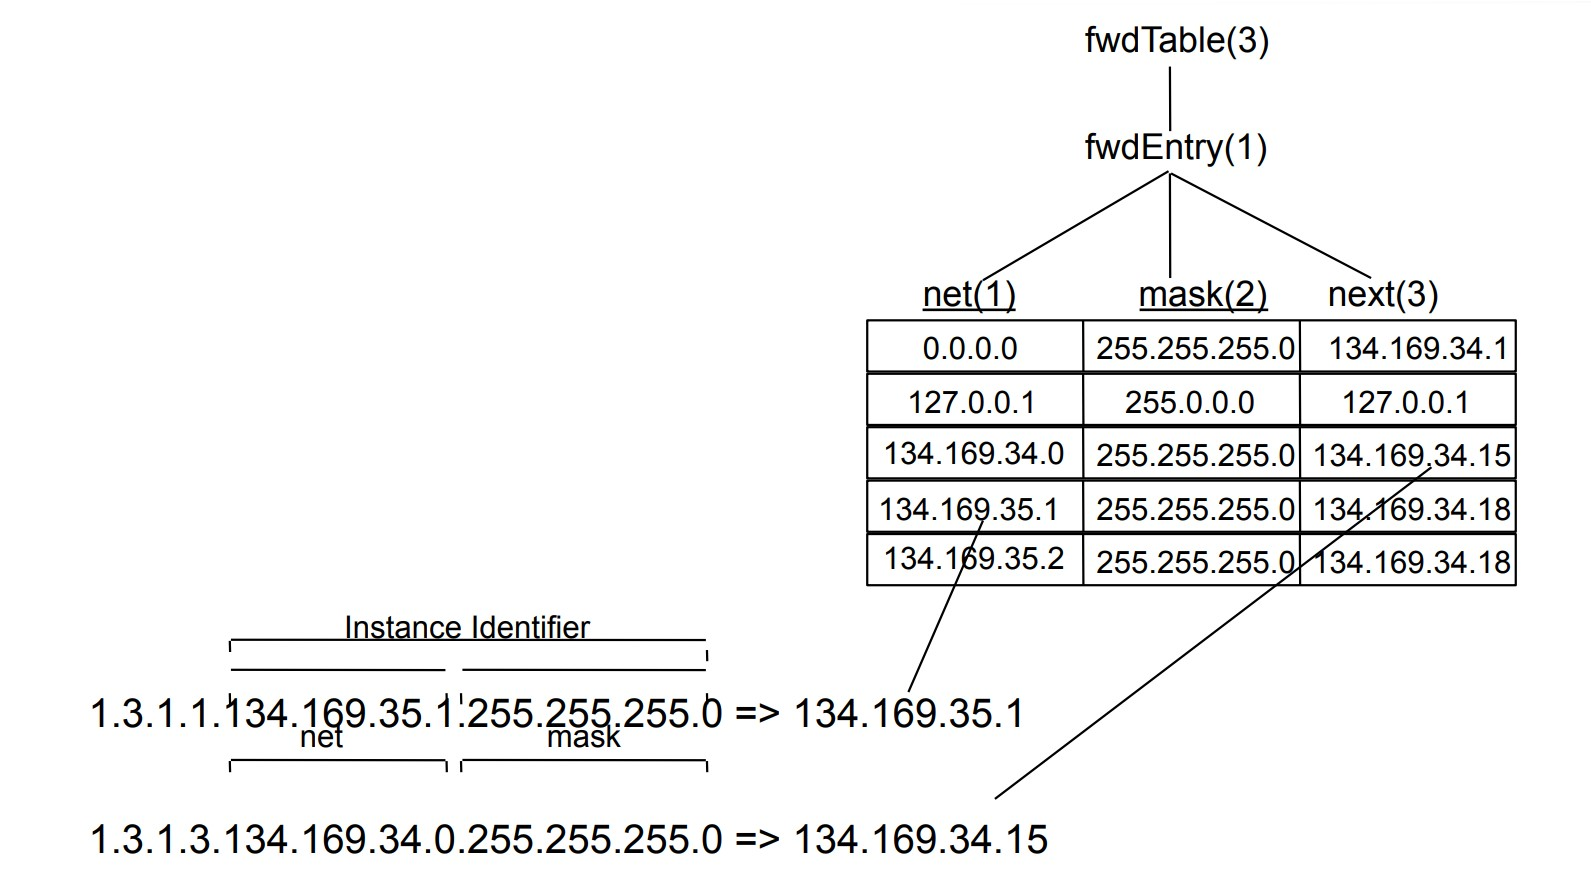
\includegraphics[width=0.9\textwidth]{immagini/RoutingTable.jpg}
\end{figure}

\subsubsection{Rules for the Specification of Instance Identifier values}

Valori per tipi fondamentali:

\begin{itemize}
    \item Valori per \texttt{INTEGER}:\ un singolo valore intero.
    \item Valori per \texttt{OCTET STRING} di lunghezza fissa:\ ogni singolo byte viene trattato come un valore individuale.
    \item Valori per \texttt{OCTET STRING} di lunghezza variabile:\ il primo valore è la lunghezza, seguita da ogni singolo byte.
    \item Valori per \texttt{OBJECT IDENTIFIER}:\ il primo valore è la lunghezza, seguita da ogni singolo byte.
\end{itemize}
La parola chiave \texttt{IMPLIED} può essere utilizzata senza il byte di lunghezza se non porta ad ambiguità.

La lunghezza massima dei valori \texttt{OBJECT IDENTIFIER} è limitata a 128 elementi, quindi gli identificatori di istanza non saranno complessi arbitrari.

\subsection{MIB Module}

Tipi di oggetti simili vengono combinati in moduli MIB,  ogni modulo MIB deve avere un nome univoco (lettere maiuscole).\
I moduli MIB sono (quasi) normali moduli ASN.1 e obbediscono alle regole lessicali ASN.1.\
Le definizioni possono essere importate da altri moduli MIB con l'aiuto dell'istruzione \texttt{IMPORT}; tutte le macro ASN.1 SMI utilizzate devono essere importate esplicitamente.

\begin{verbatim}
COFFEE-MIB DEFINITIONS ::= BEGIN

IMPORT      MODULE-IDENTITY, OBJECT-TYPE, enterprises,
            IpAddress, TimeTicks    FROM SNMPv2-SMI;
...
END
\end{verbatim}

\subsubsection{Module-Identities (RFC 2578)}

\begin{verbatim}
<descriptor> MODULE-IDENTITY
        LAST-UPDATED <ExtUTCTime>
        ORGANIZATION <Text>
        CONTACT-INFO <Text>
        DESCRIPTION <Text>
        [REVISION <ExtUTCTime>
        DESCRIPTION <Text>]*
        ::= <ObjectIdentifier>
\end{verbatim}
Definisce le informazioni amministrative, ad es.\ informazioni di contatto e numero di versione.\
Le clausole \texttt{REVISION} e \texttt{DESCRIPTION} non sono obbligatorie e possono ripetersi più volte.

\begin{figure}[H]
    \centering
    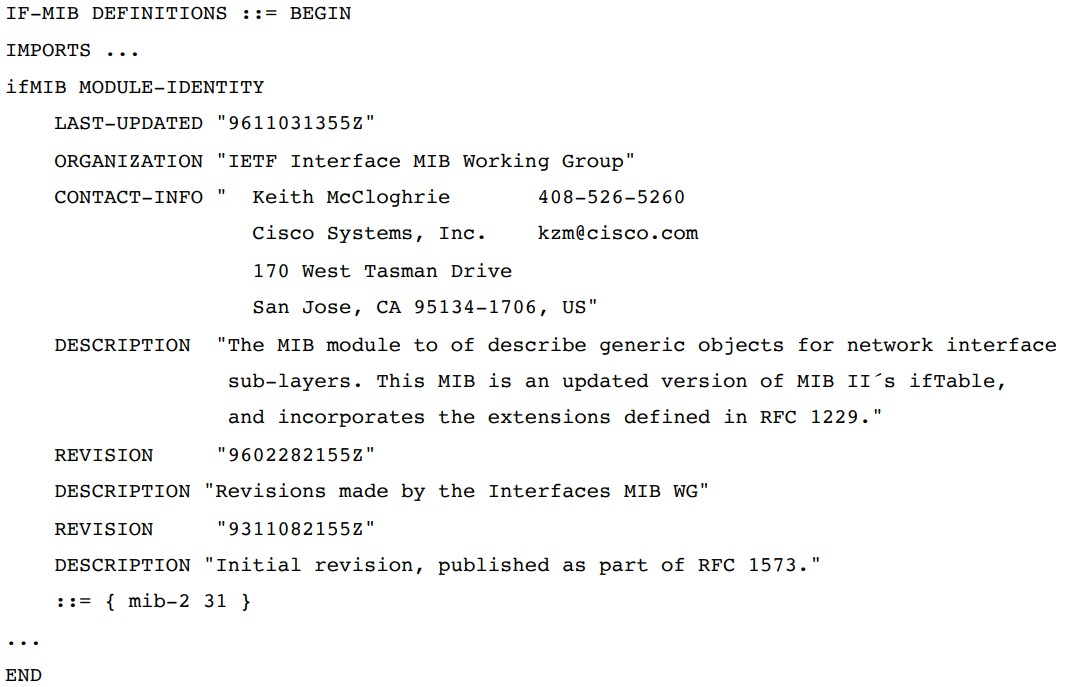
\includegraphics[width=\textwidth]{immagini/Module_Identities.jpg}
    \caption*{Esempio di Module Identities}
\end{figure}

\subsubsection{Object Identities (RFC 2578)}

\begin{verbatim}
<descriptor> OBJECT-IDENTITY
        STATUS <Status>
        DESCRIPTION <Text>
        [REFERENCE <Text>]
        ::= <ObjectIdentifier>

\end{verbatim}
Definisce e registra un valore dell'identificatore di oggetto:\ consente l'allocazione di qualsiasi nodo all'interno dell'albero di registrazione.\

La clausola \texttt{STATUS} definisce se il nodo allocato è ``obsoleto'', ``corrente'' o ``deprecato''.\
Il \texttt{REFERENCE} opzionale viene utilizzato per fare riferimento a ulteriori informazioni (simile ai collegamenti ipertestuali HTML).

\begin{figure}[H]
    \centering
    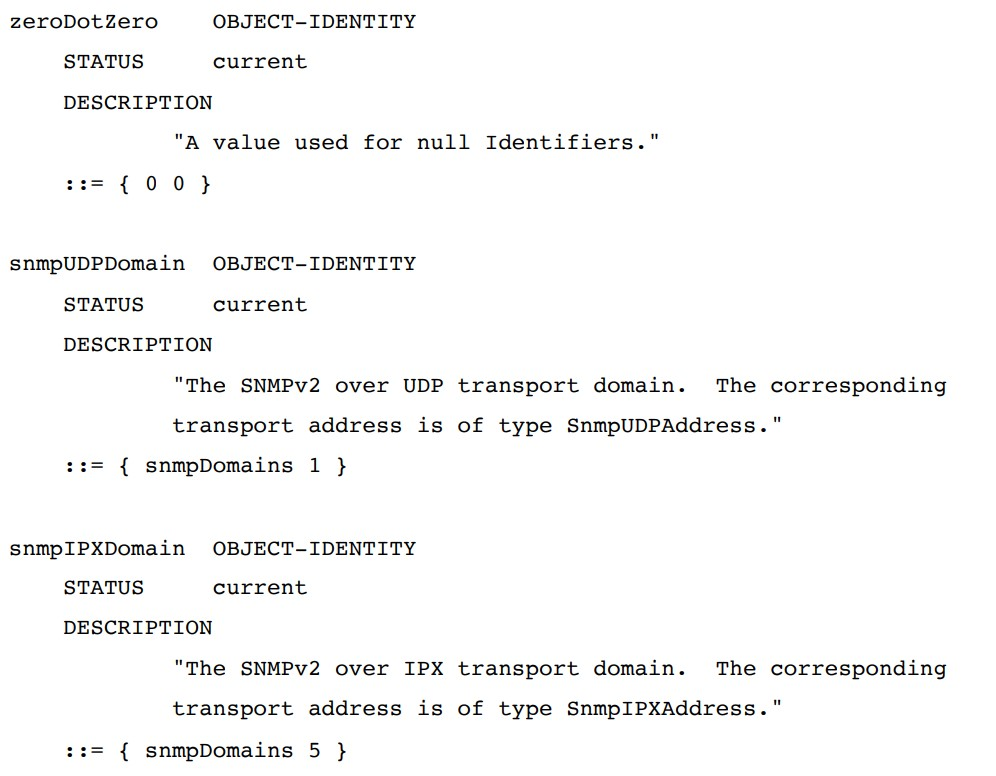
\includegraphics[width=\textwidth]{immagini/ObjectIdentities.jpg}
    \caption*{Esempio di Object Identities}
    \label{fig:my_label}
\end{figure}

\subsubsection{Object Types (RFC 2578)}

\begin{verbatim}
<descriptor> OBJECT-TYPE
        SYNTAX <Syntax>
        [UNITS <Text>]
        MAX-ACCESS <Access>
        STATUS <Status>
        DESCRIPTION <Text>
        [REFERENCE <Text>]
        [INDEX <Index>]
        [AUGMENTS <Index>]
        [DEFVAL <Value>]
        ::= <ObjectIdentifier>
\end{verbatim}
Macro per la definizione di tipologie di oggetti e tabelle concettuali.

Le clausole \texttt{INDEX} e \texttt{AUGMENTS} sono consentite solo per la definizione mediante tabelle.\
Esattamente una delle clausole precedenti deve essere specificata durante la definizione della tabella.

\begin{figure}[H]
    \centering
    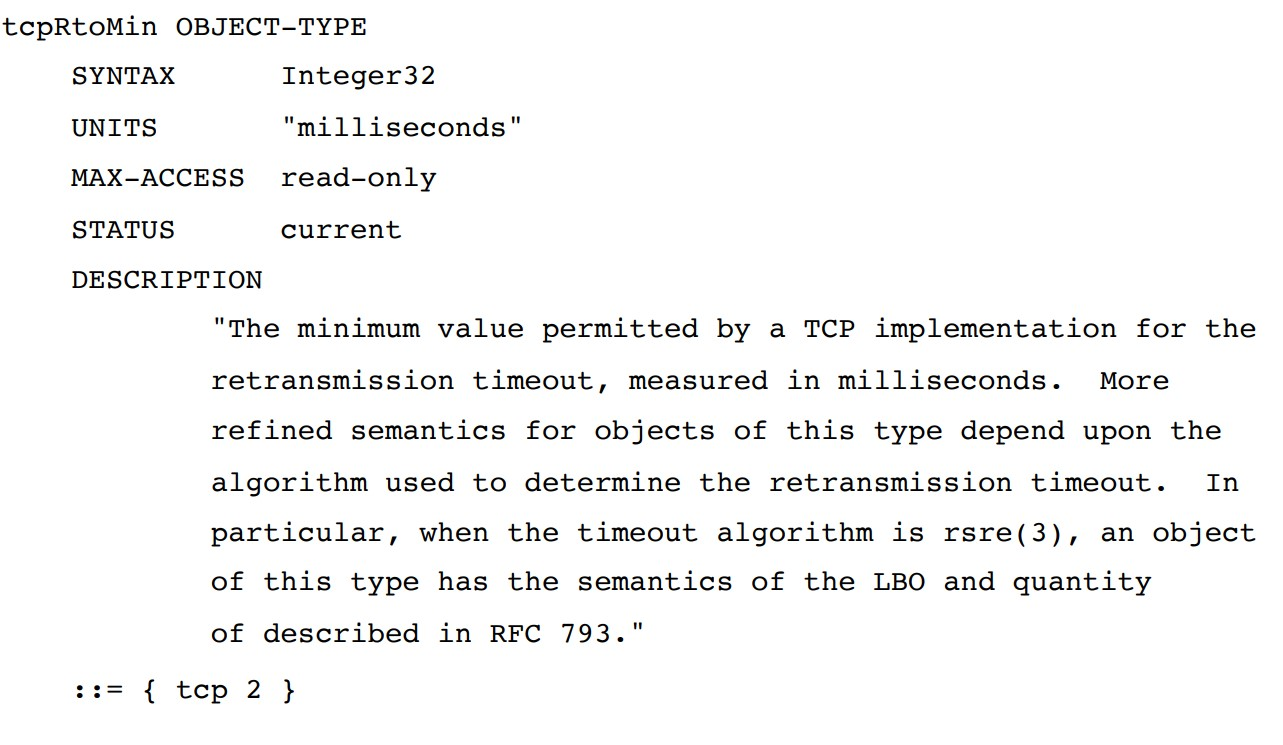
\includegraphics[width=\textwidth]{immagini/Object_Types.jpg}
    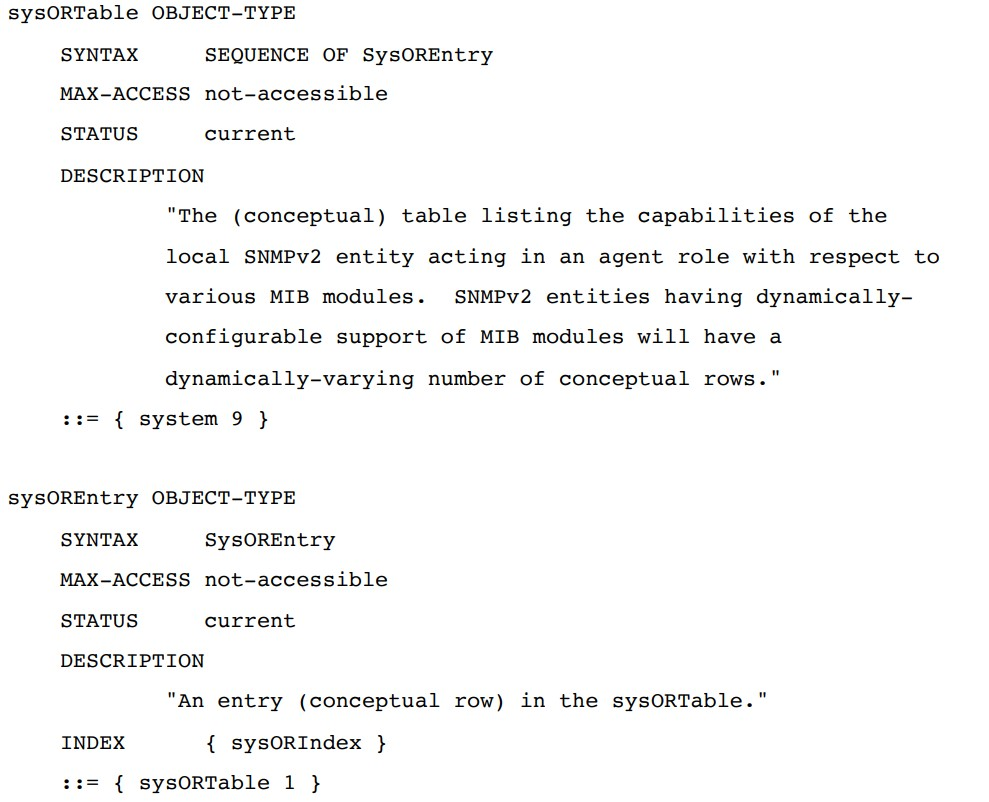
\includegraphics[width=\textwidth]{immagini/Object_Types2.jpg}
\end{figure}

\subsubsection{Notification-Types (RFC 2578)}

\begin{verbatim}
<descriptor> NOTIFICATION-TYPE
        [OBJECTS <Objects>]
        STATUS <Status>
        DESCRIPTION <Text>
        [REFERENCE <Text>]
        ::= <ObjectIdentifier>
\end{verbatim}

\noindent Macro per la registrazione di un evento; in caso di evento, un manager o un agente può inviare una notifica appropriata a un altro manager.

Le clausole \texttt{OBJECTS} definiscono quali oggetti MIB devono essere contenuti nella descrizione dell'evento.\
La clausola \texttt{DESCRIPTION} deve descrivere quali istanze si intendono caso per caso.

\subsubsection{New Types from Textual Conventions}

In SNMP non si possono definire nuovi tipi di dato, per questa ragione si utilizza la \textbf{textual convention} ridefinendo tipi di dato già esistenti per definire un tipo di dato dal punto di vista della rappresentazione.\
Tuttavia, altri tipi potrebbero non essere derivati da una \textit{textual convention}.\
Una clausola \texttt{DISPLAY-HINT} definisce una semplice figura della rappresentazione ASN.1 di un valore in un formato leggibile per gli esseri umani.\
La clausola \texttt{DISPLAY-HINT} può essere utilizzata solo insieme al tipo di dati \texttt{INTEGER} e \texttt{OCTET STRING} e da cui deriva.\

Si noti che una \textit{textual convention} può determinare restrizioni sull'ambito e non può definire un tipo assemblato.

Le convenzioni testuali sono definite nella RFC 2579.
\begin{verbatim}
<descriptor> ::= TEXTUAL-CONVENTION
        [DISPLAY-HINT <Text>]
        STATUS <Status>
        DESCRIPTION <Text>
        [REFERENCE <Text>]
        SYNTAX <Syntax>
\end{verbatim}

\noindent La clausola \texttt{DISPLAY-HINT} definisce una figura bidirezionale della rappresentazione utilizzata internamente su una rappresentazione leggibile per gli esseri umani.\
Nella clausola \texttt{SYNTAX} possono essere utilizzati solo tipi di dati di base (si possono quindi limitare ulteriormente le convenzioni testuali non esistenti).

Tutte le altre semantiche devono essere definite nella clausola \texttt{DESCRIP\-TION}.

\subsubsection{Further SMIv2 Macros}

SMI definisce delle macro su ASN.1 che permettono di raggruppare gli oggetti tra di loro.\
Quando si creano dei MIB, è possibile che i vari oggetti implementino solo una parte dell'intera funzionalità.\
Queste macro hanno la possibilità di dividere gli oggetti in gruppi, così facendo sarà presente un \textbf{gruppo minimo}, ovvero il modulo del dispositivo che permetterà a quest'ultimo di essere conforme alla specifica.

\begin{itemize}
    \item \texttt{OBJECT-GROUPS}:\ consente la definizione di gruppi di tipi di oggetti correlati; questa macro può essere utilizzata nella macro \texttt{MODULE-COMPLI\-ANCE}.
    \item \texttt{NOTIFICATION-GROUPS}:\ consente la definizione di gruppi di tipi di notifica correlati; questa macro può essere utilizzata nella macro \texttt{MOD\-ULE-COMPLIANCE}.
    \item \texttt{MODULE-COMPLIANCE}:\ definisce uno o più vincoli che le implementazioni MIB devono soddisfare.
    \item \texttt{AGENT-CAPABILITIES}:\ descrive le capacità di un'implementazione MIB reale.
\end{itemize}

\subsection{MIB-Compiler}

\begin{figure}[H]
    \centering
    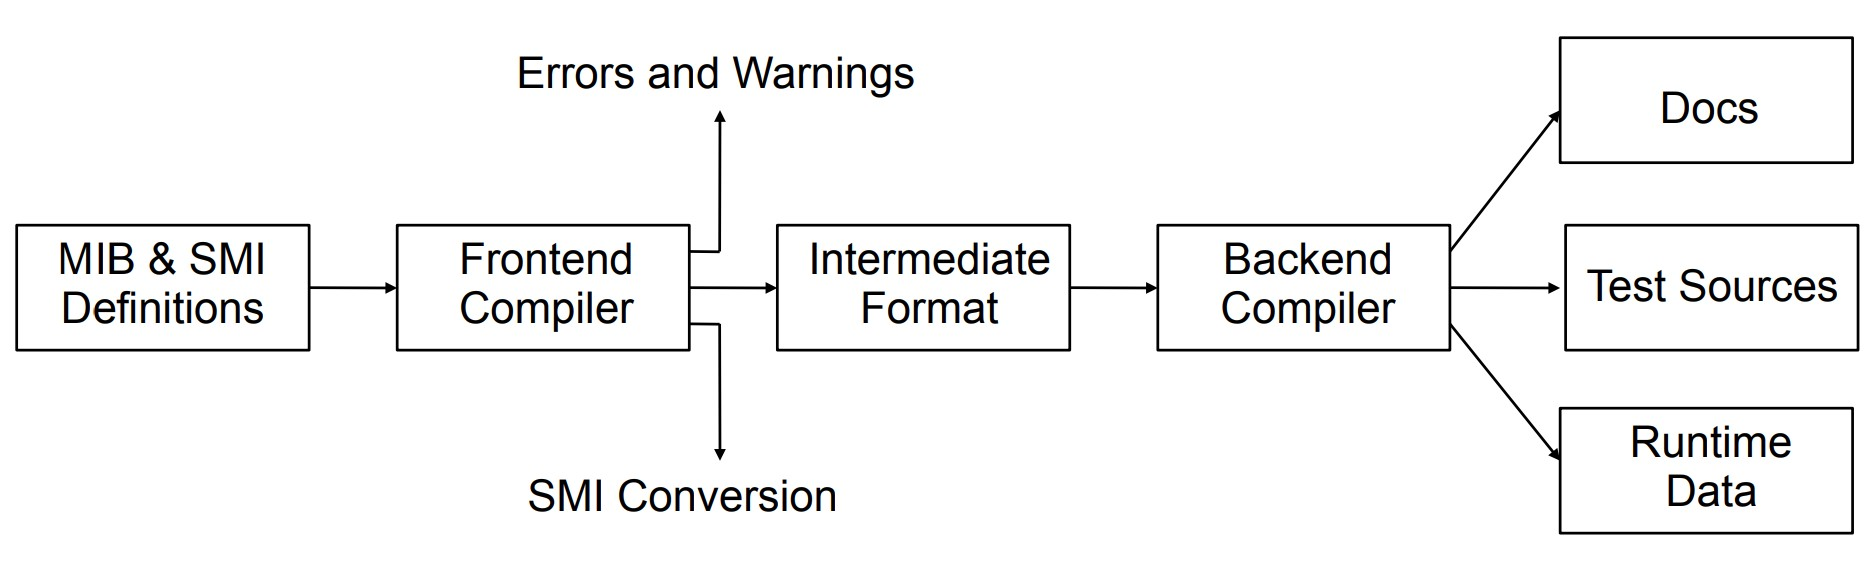
\includegraphics[width=\textwidth]{immagini/MIB_Compiler.jpg}
\end{figure}

Gli oggetti una volta definiti vengono scritti in formato testuale sul file system e possono essere utilizzati per più fini.\
Prima di eseguire una conversione di formato avviene una \textit{verifica formale} allo scopo di verificare l'assenza di problemi; questa operazione risulta particolarmente utile nelle fasi di \texttt{IMPORT} da un altro oggetto.\
Se la verifica formale va a buon fine si ottiene una rappresentazione intermedia per il backend-compiler, il quale può produrre la documentazione (utilizzando le descrizioni presenti nei notification typer, object identities, \dots), dei test case per verificare se l'implementazione è corretta (se ho una variabile definita come read-only, il test deve fallire in caso si provi a fare una scrittura) e i run time data (generati dopo la lettura dei dati).

\textbf{Osservazione}:\ non esiste un formato intermedio standardizzato o generalmente accettato.

\section{Fundamental MIBs}

MIB-II (RFC 1213) definisce i tipi di oggetto per i protocolli Internet IP, ICMP, UDP, TCP, SNMP (e altre definizioni non rilevanti qui); fondamentalmente modella la gestione dello stack del protocollo TCP/IP.\
La definizione MIB-II ha come obiettivi definire gli errori di base e la gestione della configurazione per i protocolli Internet, evitare informazioni ridondanti nel MIB e avere pochissimi e deboli oggetti di controllo.\
Inoltre, l'implementazione del MIB non dovrebbe interferire con le normali attività di rete e nessun tipo di oggetto deve dipendere da essa.

Complessivamente 170 tipi di oggetti:\ alcune definizioni MIB si sono rivelate troppo semplici e minime (tabella di instradamento, tabella di interfaccia), mentre altre presuppongono un formato di indirizzo a 4 byte, quindi queste tabelle devono essere ridefinite per IP versione 6 (IPv6).

\begin{figure}[H]
    \centering
    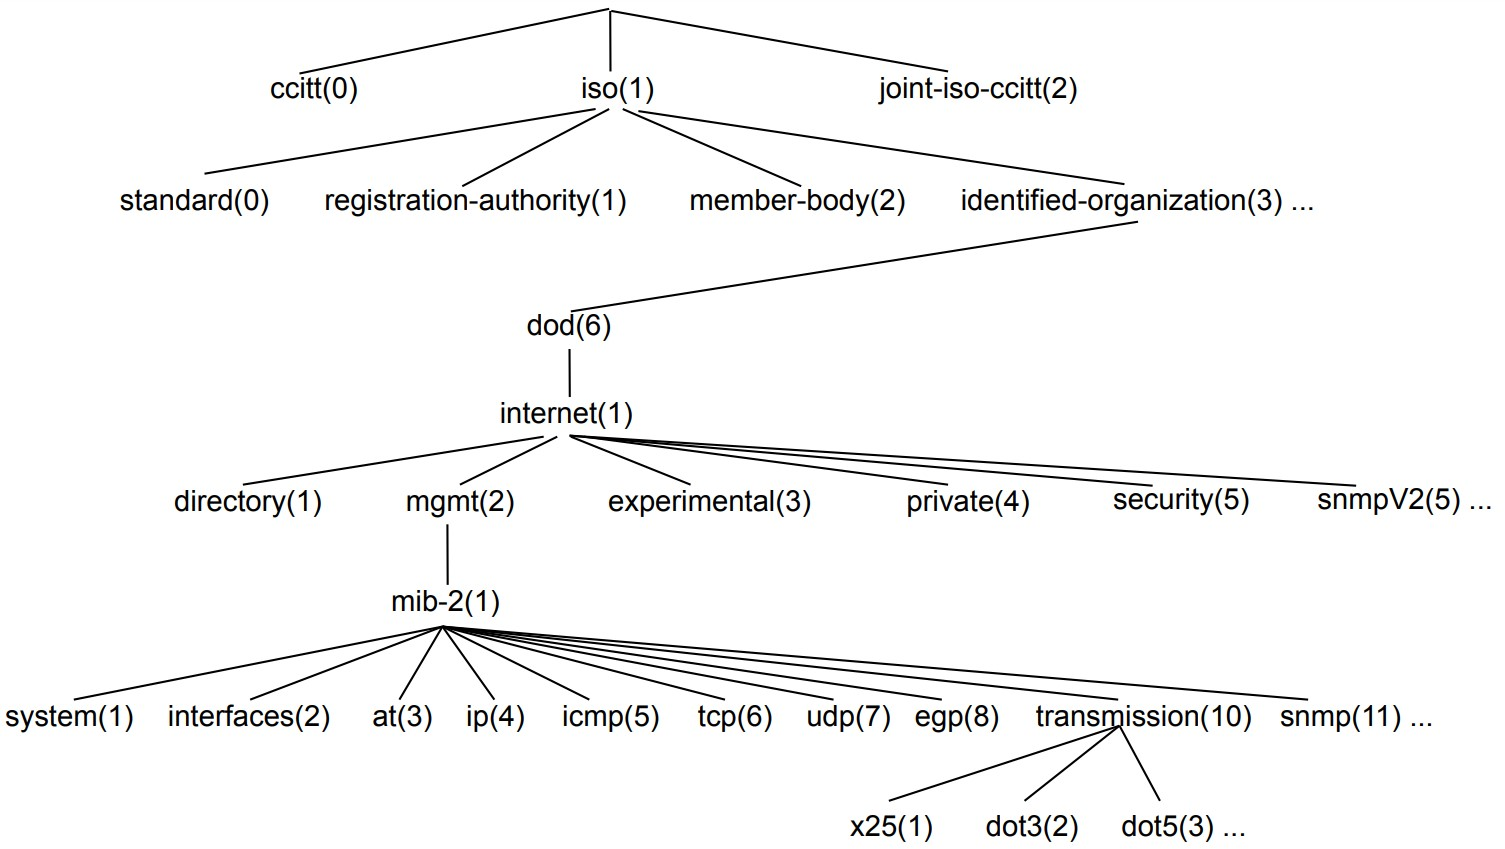
\includegraphics[width=\textwidth]{immagini/StructureMIBII.jpg}
\end{figure}

\noindent Il MIB-II è uno dei più importanti perché è nato con SNMP ed ha portato alla diffusione di quest'ultimo:\ il protocollo http è utile fin tanto che ci sono siti web da leggere, MIB-II funge da sito web, infatti all'interno di quest'ultimo sono presenti le informazioni di monitoraggio da analizzare con SNMP.\
Infine, MIB-II è importante perché permette di gestire tutte quelle che sono le informazioni di base di un sistema basato su SNMP (informazioni sulle interfacce di rete, sull'ARP table, sul protocollo IP, sull'ICMP, \dots).

\subsubsection{Osservazioni su MIB-II}

\begin{itemize}
    \item Il ramo ``\texttt{transmission}'' ospita tutte le definizioni MIB che si occupano della trasmissione delle informazioni (X.25, PPP, RS232, SONET, ISDN, IEEE 802.3, IEEE 802.5, FDDI,\ \dots)
    \item Il ramo ``\texttt{at}'' (ARP Table) è stato sostituito da un'estensione del gruppo di IP.
    \item Il ramo \texttt{egp} (External Gateway Protocol) non è più utilizzato in quanto il protocollo EGP al giorno d'oggi non ha alcuna importanza.
    \item Molti altri moduli MIB sono stati registrati nel nodo ``\texttt{mib-2}''.\ L'assegnazione dei numeri di registrazione è delegata allo IANA (Internet Assigned Numbers Authority).
    \item In questi giorni sarebbe bene introdurre una certa modularità nel MIB in modo che i diversi rami possano essere aggiornati in modo indipendente.\
\end{itemize}

\section{SNMP Version 1}

\begin{figure}[H]
    \centering
    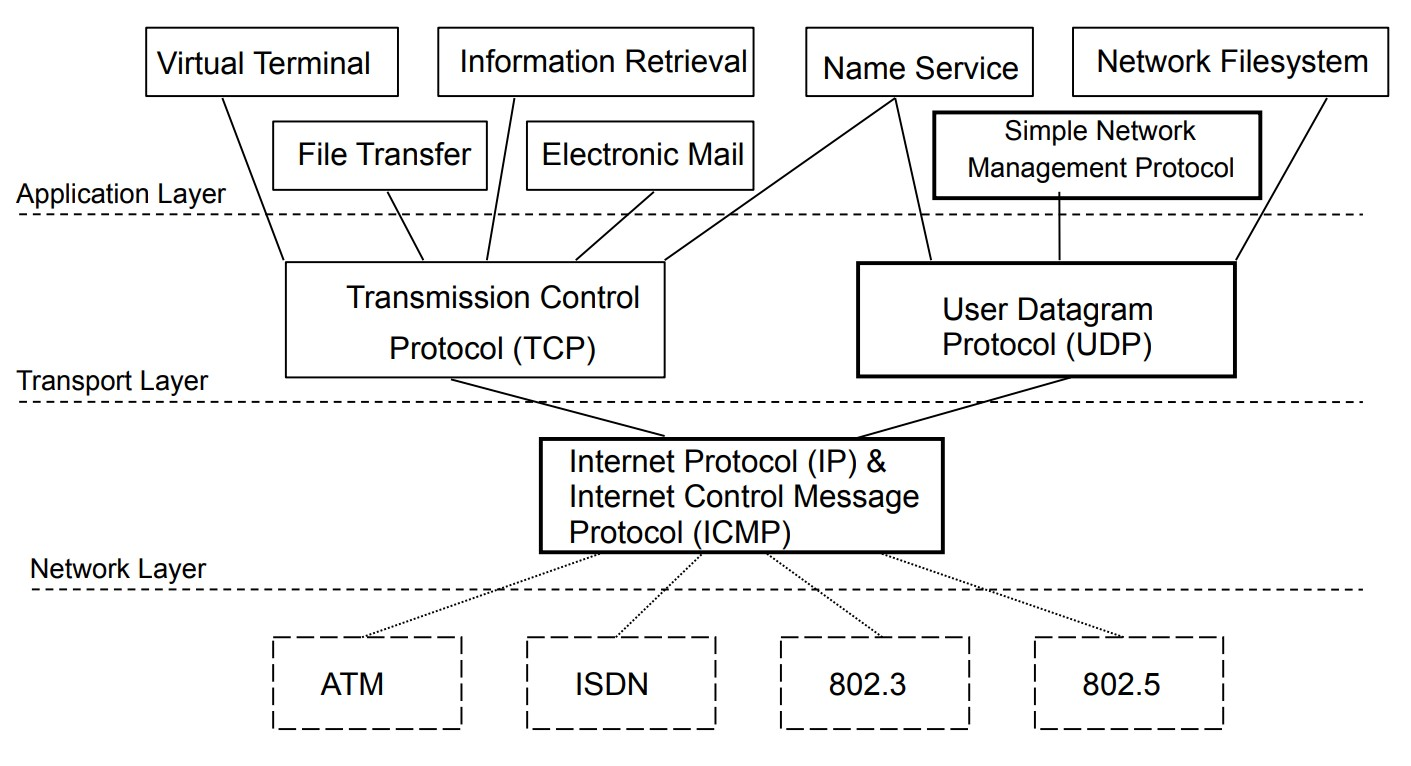
\includegraphics[width=0.9\textwidth]{immagini/SNMP.jpg}
\end{figure}

\textbf{SNMP} (\textit{Simple Network Management Protocol}) si trova nella parte alta dello stack TCP{\slash}IP, nell'Application Layer.\
Nel caso del mondo ISO{\slash}OSI corrisponde al livello 7, dove si trovano le applicazioni usate dagli utenti.\

È un protocollo che sfrutta \textbf{UDP} come servizio del livello di transporto, perciò si tratta di un protocollo \textit{connectionless}.\
In realtà esiste anche una versione che supporta il protocollo TCP, tuttavia si privilegia quella che fa uso di UDP.\

\subsubsection{Ordinamento lessicografico}

Le istanze MIB sono disposte nel MIB lessicograficamente in base al valore dell'identificatore di oggetto che identifica l'istanza.\
Il registro SNMP utilizza questa caratteristica per leggere (\textit{walk}) tabelle concettuali o MIB sconosciuti.\

\begin{table}[H]
    \centering
    \begin{tabular}{|l|l|l|l|}
        \hline
        \textbf{Object Identifier} & \textbf{Value}  & \textbf{Object Identifier} & \textbf{Value} \\\hline \hline
        1.1.0                      & 10.1.2.3        & 1.3.1.2.3                  & 5              \\
        1.2.1.0                    & ``FilterFresh'' & 1.3.1.2.4                  & 7              \\
        1.2.2.0                    & 54321           & 1.3.1.2.5                  & 8              \\
        1.3.1.1.1                  & 1               & 1.3.1.2.6                  & 9              \\
        1.3.1.1.2                  & 2               & 1.3.1.3.1                  & 2              \\
        1.3.1.1.3                  & 3               & 1.3.1.3.2                  & 3              \\
        1.3.1.1.4                  & 4               & 1.3.1.3.3                  & 2              \\
        1.3.1.1.5                  & 5               & 1.3.1.3.4                  & 2              \\
        1.3.1.1.6                  & 6               & 1.3.1.3.5                  & 3              \\
        1.3.1.2.1                  & 2               & 1.3.1.3.6                  & 3              \\
        1.3.1.2.2                  & 3               &                            &                \\\hline
    \end{tabular}
    \caption*{Esempio di ordinamento lessicografico}
\end{table}

\noindent Con questo ordinamento la struttura concettuale della tabella viene persa poiché l'output del percorso è un elenco e non più una tabella.\

Il protocollo SNMP opera solo su questo elenco organizzato.

\subsubsection{SNMPv1 operations}

Le primitive principali di SNMPv1 sono
\begin{table}[H]
    \centering
    \begin{tabular}{l l}
        \texttt{get}     & legge il valore di un Object Identifier                            \\
        \texttt{getNext} & legge il valore dell'Object Identifier successivo a quello attuale \\
        \texttt{set}     & imposta il valore relativo a un Object Identifier                  \\
        \texttt{trap}    & manda una notifica al manager                                      \\
    \end{tabular}
\end{table}

\noindent Le prime tre operazioni sono sempre ``iniziate'' dal manager, la \texttt{trap} è l'unica che permette all'agent di contattare il manager:\ è necessaria per mandare una notifica relativa a un cambio di stato al manager poiché usare il \textit{polling} sarebbe poco efficiente (poco scalabile) e poco sicuro.\
Se si utilizzassero solo le trap senza il ciclo di polling, nessuno controllerebbe che gli agent abbiano svolto correttamente il loro lavoro e il loro funzionamento (operazione che in origine era affibbiata al manager mediante il polling).\
In SNMP c'è il problema di \textbf{agent unreachable}:\ il manager pensa che stia andando tutto bene, mentre l'agent sta cercando di mandargli messaggi informativi che però non arrivano a causa di un guasto alla rete.\

L'approccio SNMP è sensato se il numero di dispositivi (agent) da controllare è piccolo; se la quantità di dispositivi da monitorare è molto grande, c'è la necessità di arricchire le trap da parte degli agent rendendole più potenti:\ per esempio, nel caso di uno switch a 48 porte, la trap deve coprire lo spazio di gestione di tutte le porte.\

\begin{figure}[H]
    \centering
    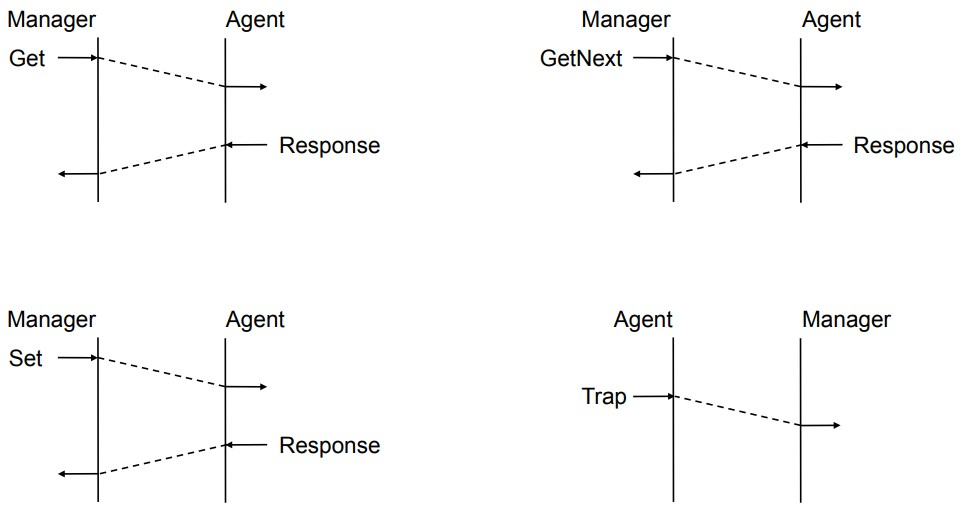
\includegraphics[width=0.9\textwidth]{immagini/SNMP_operations.jpg}
\end{figure}

\noindent\textbf{Nota}:\ il protocollo SNMP può scambiare solo (un elenco di) scalari.

\subsection{Formato messaggi SNMPv1}

Il primo campo dei messaggi SNMP contiene la \textit{versione}.\
Il secondo campo contiene una stringa, \textit{community}, usata per l'autenticazione degli utenti (controllo sui diritti, come una password).

\begin{figure}[H]
    \centering
    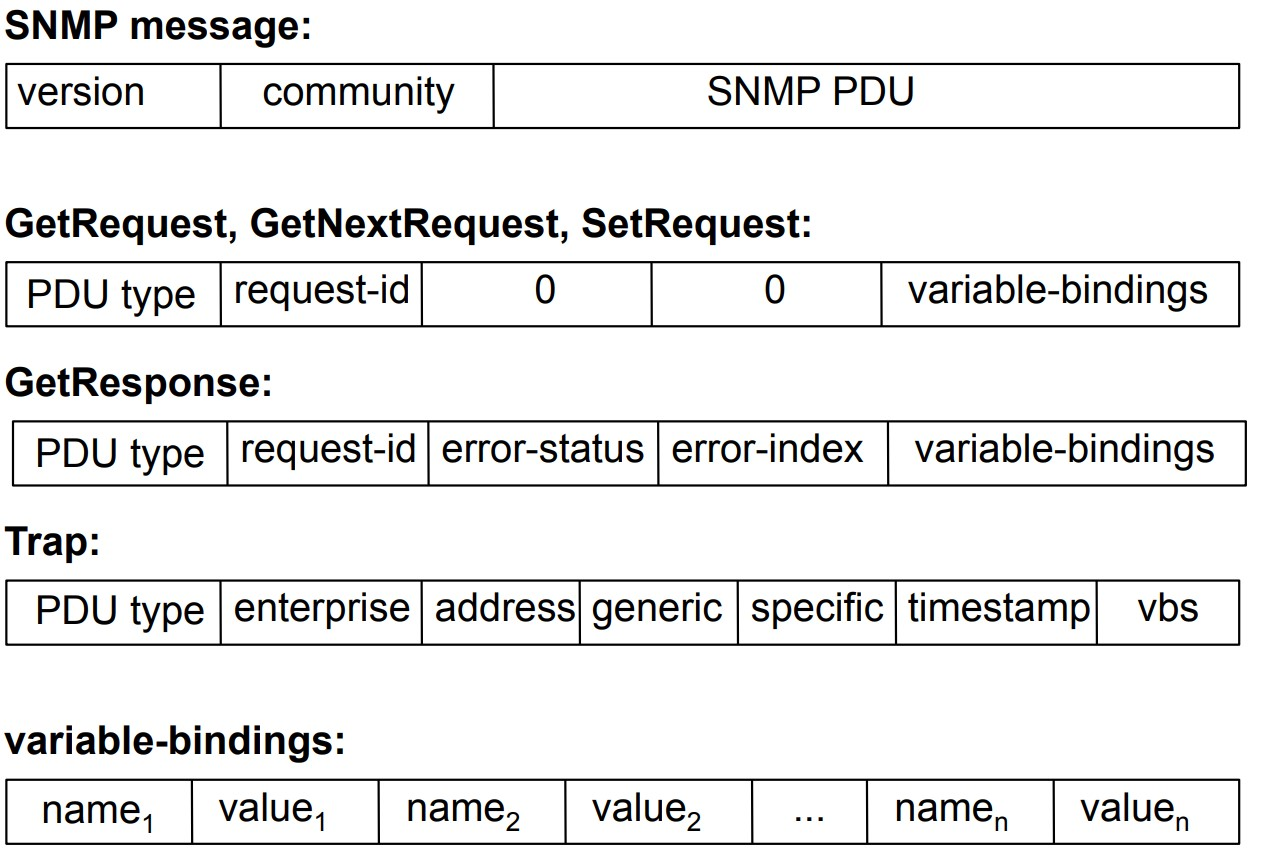
\includegraphics[width=0.8\textwidth]{immagini/SNMP_messageFormat.jpg}
\end{figure}

\noindent Infine vi è il \textbf{PDU} (\textit{Protocol Data Unit}) che varia a seconda del tipo di messaggio.\ Nel caso della request la \texttt{get}, la \texttt{getNext} e la \texttt{set} contengono un'identificativo unico della richiesta usato per ``legare'' la successiva risposta e un campo contenente una serie di \verb|<Object Identifier, valore>|:\ $\simeq$ 1400 byte a disposizione, nel caso in cui si sfori tale dimensione l'invio del messaggio fallisce e viene generato un codice di errore specifico.\ La \texttt{trap} ha un formato diverso.\

All'inizio di ogni PDU vi è un campo \texttt{type} per distinguere il tipo di messaggio.\

\textbf{Osservazione}:\ l'agent gestisce le richieste in modo atomico (una richiesta per volta), quelle che vengono ricevute e che non possono essere elaborate vengono accodate.\
Se le primitive vengono eseguite su un singolo object-ID piuttosto che su un insieme si perde la proprietà di atomicità (le richieste in questo caso vengono gestite come nei programmi multithreaded).

\subsubsection{Get Operation}

L'operazione \texttt{get} può essere utilizzata per leggere una o più variabili.\
Possibili errori durante l'elaborazione di un'operazione \texttt{get}:
\begin{table}[H]
    \centering
    \begin{tabular}{l l}
        \texttt{noSuchName} & l'istanza richiesta non esiste o non è una foglia             \\
        \texttt{tooBig}     & il risultato della richiesta non rientra nella risposta (UDP) \\
        \texttt{genErr}     & si è verificato qualsiasi altro errore                        \\
    \end{tabular}
\end{table}

\noindent In caso di più errori, solo un errore viene segnalato come indice di errore e stato di errore sono univoci nella PDU.

\subsubsection{GetNext Operation}

Recupera il nome dell'oggetto e il valore dell'istanza successiva, viene utilizzata per rilevare le strutture MIB e leggere le tabelle.\

\texttt{getNext} consente di leggere le istanze MIB secondo l'ordine lessicografico:\ utilizzando più{\slash}successive operazioni \texttt{getNext} è possibile leggere l'intero MIB senza conoscerne la struttura.\
Possibili errori durante l'elaborazione di un'operazione \texttt{getNext}:

\begin{table}[H]
    \begin{tabular}{l l}
        \texttt{noSuchName} & l'istanza richiesta non esiste (= fine del MIB)               \\
        \texttt{tooBig}     & il risultato della richiesta non rientra nella risposta (UDP) \\
        \texttt{genErr}     & si è verificato qualsiasi altro errore                        \\
    \end{tabular}
\end{table}

\subsubsection{Set Operation}

L'operazione di \texttt{set} scrive i valori in una o più istanze MIB atomicamente.\
Con l'aiuto dell'operazione \texttt{set} è possibile creare anche nuove istanze MIB, se la definizione MIB lo consente (non esiste una procedura standard definita in SNMPv1 per la creazione dell'istanza).\
Possibili errori durante l'elaborazione di un'operazione \texttt{set}:

\begin{table}[H]
    \begin{tabular}{l l}
        \texttt{noSuchName} & l'istanza richiesta non esiste e non può essere creata        \\
        \texttt{badValue}   & il valore specificato è di tipo sbagliato                     \\
        \texttt{tooBig}     & il risultato della richiesta non rientra nella risposta (UDP) \\
        \texttt{genErr}     & si è verificato qualsiasi altro errore                        \\
    \end{tabular}
\end{table}

\noindent Viene definito anche il codice di errore \texttt{readOnly}, ma generalmente non viene usato.

\subsubsection{Trap Operation}

Con l'operazione \texttt{trap} gli agents possono informare un manager riguardo un evento; poiché non si vogliono mischiare i traffici di \texttt{get} e \texttt{set} con quelli di \texttt{trap}, in questo caso si usa la porta 162.\

Per ricevere queste trap, il Manager deve avere un demone sulla porta 162 che resta in ascolto e le gestisce.\
Nel caso più comune, se non vi è nessuno ad ascoltare il traffico in arrivo o la macchina è spenta, i pacchetti vengono persi.\ Nel caso meno comune vengono comunque persi ma viene anche inviato un messaggio ICMP \texttt{destination unreachable} alla sorgente dei messaggi.\
\textbf{Nota}:\ un manager può essere configurato per ignorare le traps!\

La ricezione di un'operazione \texttt{trap} non è riscontrata, quindi non è affidabile in quanto può essere persa durante il trasferimento.\
La generazione di traps può portare alle cosiddette ``\textit{trap storm}'', ad esempio se dopo un'interruzione di corrente tutti i dispositivi vogliono visualizzare contemporaneamente il riavvio.\
Gli agenti possono essere normalmente configurati con gli indirizzi IP degli host in cui è possibile inviare trap, tuttavia non esiste una tecnica standard in SNMPv1 per tale configurazione dell'agente:\ di solito viene utilizzato un file di configurazione (non il MIB).\
Sebbene si utilizzino le traps, il polling è ancora necessario (ad esempio, l'agente potrebbe essere inattivo).\

\section{SNMP Version 2c}

Il termine SNMPv2 è ambiguo.\
SNMPv2c doveva risolvere i problemi della v1 tra cui l'autenticazione; la sola presenza della \textit{comunità} come misura di sicurezza (che passava in chiaro) non era abbastanza considerando che al tempo venivano usati gli hub:\ il traffico veniva mandato ovunque nelle reti locali ed era quindi molto semplice reperire la ``password'' da usare per eseguire primitve SNMP.\
Esistono alcune varianti di SNMP versione 2:
\begin{itemize}
    \item SNMPv2p:\ Versione con modello di sicurezza basato sulle parti, storico.
    \item SNMPv2c:\ SNMPv2 con banale modello di sicurezza basato sulla comunità, sperimentale.
    \item SNMPv2u:\ SNMPv2 con un modello di sicurezza basato sull'utente, storico.
    \item SNMPv2*:\ SNMPv2 con modello di sicurezza e amministrazione, storico.
\end{itemize}
Ci furono varie proposte ma il loro sviluppo andava per le lunghe quindi la community venne lasciata e SNMPv2 diventò SNMPv2c.\
Quest'ultimo ha riscontrato una certa diffusione, sebbene IETF non lo abbia mai standardizzato.\

Sono state aggiunte le \textbf{eccezioni}, le quali consentono di segnalare gli errori di accesso alle istanze alle autorità MIB, senza causare il fallimento dell'intera operazione (come accadeva in SNMPv1), e due nuove primitive:\ \texttt{getBulk}, per velocizzare lo scorrimento di tabelle, e \texttt{inform} che si comporta da \texttt{trap} confermata.\

\begin{table}[H]
    \centering
    \begin{tabular}{|l|l|l|}
        \hline
        SNMPv2 Exception        & SNMPv1 Status       & Used by                            \\\hline\hline
        \texttt{noSuchObject}   & \texttt{noSuchName} & \texttt{Get}                       \\
        \texttt{noSuchInstance} & \texttt{noSuchName} & \texttt{Get}                       \\
        \texttt{endOfMibView}   & \texttt{noSuchName} & \texttt{GetNext}, \texttt{GetBulk} \\\hline
    \end{tabular}
    \caption*{SNMPv2 Exceptions (RFC 1905)}
\end{table}

\subsubsection{Get and GetNext Operations}

Le istanze MIB non esistenti producono un'eccezione e non un errore.\
Simile alle operazioni SNMPv1 equivalenti.

\subsubsection{Set Operation}

Ci sono 14 possibili codici di errore durante l'elaborazione delle operazioni di \texttt{set}:
\begin{table}[H]
    \centering
    \begin{tabular}{l l l}
        \texttt{wrongValue}          & \texttt{wrongEncoding}     & \texttt{wrongType}        \\
        \texttt{wrongLength}         & \texttt{inconsistentValue} & \texttt{noAccess}         \\
        \texttt{notWritable}         & \texttt{noCreation}        & \texttt{inconsistentName} \\
        \texttt{resourceUnavailable} & \texttt{commitFailed}      & \texttt{undoFailed}       \\
    \end{tabular}
\end{table}

\noindent Ci sono altri due codici di errore che sono stati definiti ma non utilizzati realmente: \texttt{readOnly} e \texttt{permissionError}.\
Nessun supporto di codici di errore il tipo di oggetto.\

\subsubsection{GetBulk Operation}

\texttt{getBulk} è stata introdotta per supplire ai problemi di \texttt{getNext} \textbf{velocizzando lo scorrimento} di tabelle.\
Scorrere una tabella con \texttt{getNext} implica dover fare una richiesta, attendere la risposta, inserire l'OID della risposta in una nuova richiesta\dots\ quindi per \textit{n} righe di tabelle, si eseguono \textit{n} \texttt{getNext} e, nel caso di host remoto, ci sarà un po' di latenza che renderà questo lungo; quindi, nella \texttt{getBulk} è stata inserita la possibilità di ricevere più righe di risposta per una singola richiesta e non solo:\ è stato pensato anche di unire \texttt{get} e \texttt{getNext}.\
La \texttt{getBulk} ha il seguente formato:
\begin{center}
    \verb|getBulk(non-repeaters=n, max-repetitions=m, OID)|
\end{center}

\noindent Il parametro \texttt{non-repeaters} indica quanti OID di quelli specificati richiedono una \texttt{get} (normale), al resto dei parametri \textit{verrà applicata una} \texttt{getNext} \textit{in automatico}.\
Il parametro \texttt{max-repetitions} indica quante \texttt{getNext} eseguire sugli OID che non hanno richiesto una \texttt{get}.\

\textbf{Nota}:\ qualora la tabella su cui si esegue la \texttt{getBulk} sia più piccola di \texttt{max-repetitions}, verranno ritornati tutti e soli i valori della tabella.\
Quindi, con una sola richiesta-risposta è possibile fare fino a \textit{n} \texttt{getNext} e ciò non è male poiché il numero di messaggi in rete è diminuito (più efficiente).\

Senza la conoscenza della lunghezza di una tabella è difficile per il manager selezionare un numero adatto per il numero massimo di ripetizioni:
\begin{itemize}
    \item se il numero massimo di ripetizioni è troppo piccolo, non vi è alcun aumento di efficienza di \texttt{getBulk} rispetto all'operazione \texttt{getNext};
    \item se \texttt{max-repetitions} è troppo grande, viene letto un gran numero di istanze non necessarie.
\end{itemize}

\noindent L'agente può eventualmente produrre una risposta, che può perdersi in reti grandi/occupate o non essere elaborata affatto dal gestore (questo fa sì che il gestore ritrasmetta la richiesta).\

Se il numero massimo di ripetizioni è elevato e la lettura delle istanze MIB richiede molto tempo, gli agenti possono ricevere più volte la richiesta del manager (ad esempio a causa della ritrasmissione) bloccando così l'agente per un po' di tempo.\

\subsubsection{Inform Operation}

La struttura della PDU corrisponde a quella di una \texttt{trap} SNMPv2.\
Consente ai (nuovi) gestori di parlare tra loro (interazione limitata da SNMPv1 con agente-gestore o viceversa).\
La ricezione di un messaggio \texttt{inform} viene confermata con un messaggio di risposta.\

Nella pratica non ha avuto molto successo perché i problemi non sono così semplici; se un mittente manda una \texttt{inform} e non riceve nessuna risposta, non può saperne il motivo:\ il destinatario potrebbe non averla mai ricevuta, il destinatario potrebbe aver risposto ma tale risposta si è persa oppure il destinatario potrebbe non rispondere e basta.\
Tuttavia, il problema risiede nel fatto che la \texttt{inform} complica SNMP:\ i mittenti devono ricordarsi selettivamente le \texttt{inform} alle quali non hanno ricevuto risposta e devono avere anche un timeout per ognuna di esse (i device che usano SNMP ci mettono tanto per rispondere alle \texttt{inform} in quanto il processo di SNMP non viene schedulato spesso); memorizzarsi le \texttt{inform} senza risposta è necessario per evitare che il mittente rinvii le \texttt{inform} alle quali ha ricevuto risposta.\

\textbf{Nota bene}:\ va considerato che un agent può avere più manager, quindi il numero di \texttt{inform} da memorizzare può (ipoteticamente) aumentare.\
Inoltre, anche i manager vogliono sapere se gli agent/manager hanno ricevuta la loro risposta alla \texttt{inform} quindi anche loro hanno questo problema.\
Questo problema ha decretato ``il fallimento'' della \texttt{inform} nella maggior parte dei casi.

\subsubsection{SNMPv2 vs SNMPv1}

\begin{itemize}
    \item \textbf{Gestione contatori anche a 64 bit} (meno rischio di wrap dei contatori in connessioni ad alta velocità).
    \item \texttt{getBulk} consente di \textbf{fare \textit{walk} più veloci} e diminuire il numero di richieste-risposte permettendo di fare polling di più Agent contemporaneamente.
    \item \textbf{Messaggi di errore più precisi sulle primitive}.
    \item Nuovi datatype.
    \item Introdotti nuovi protocolli di trasporto (in SNMPv3 si userà addirittura TCP).
    \item Le \texttt{trap} possono essere mandate a più manager con un solo messaggio.
\end{itemize}

\section{SNMPv3}

Obiettivi di progettazione di SNMPv3:
\begin{itemize}
    \item Emissione di operazioni \texttt{set} protette.
    \item Definizione (si spera) di un modello di architettura longeva.
    \item Supporto sia di implementazioni semplici ed economiche che complesse e più costose (scalabilità).
    \item Indipendenza dagli standard.
    \item Utilizzo di materiale esistente (principalmente MIB) quando possibile (riutilizzo del progetto).
    \item SNMP deve rimanere il più semplice possibile.
\end{itemize}

\noindent Diverse implementazioni (commerciali e open source) disponibili.\
La diffusione in reti reali è ancora relativamente piccola (la maggior parte dei dispositivi di rete utilizza ancora SNMPv1).

\subsection{Modello architetturale di SNMPv3}

Il motore SNMP di un'entità SNMP è costituito da diversi sottosistemi e un dispatcher.\
Il modello manager/agente viene sostituito da una serie di ``applicazioni'' più piccole:\ la modularità consente l'avanzamento incrementale di SNMP tramite SNMP Context (RFC 2571).

\subsubsection{SNMP Context}

Un \textit{context} è una quantità di informazioni di gestione a cui può avere accesso un'entità SNMP.\
Per ogni sottosistema un'entità SNMP ha potenzialmente accesso a diversi contesti e le stesse informazioni possono essere presenti in più contesti.\
In un dominio di gestione un'istanza di un Managed Objects è identificata in modo univoco dai seguenti elementi:
\begin{itemize}
    \item l'identificazione dei motori SNMP in un'entità SNMP;
    \item il nome del contesto in un'entità SNMP;
    \item l'identificazione del tipo di Managed Object;
    \item l'identificazione dell'istanza.
\end{itemize}

\noindent\textbf{Nota}:\ l'identificazione di un motore SNMP non ha nulla a che fare con il loro indirizzamento.

Per rendere l'architettura a lungo termine hanno cambiato il trasporto e aggiunto nuovi protocolli ma soprattutto hanno deciso che ogni volta che si fosse implementata una nuova versione, sarebbe stato scelto il nuovo eventuale componente da linea di comando al momento della richiesta.\
Per la sicurezza invece è stato aggiunto il modello \verb|username-psw| e hanno lasciato aperta la possibilità di un nuovo modello (sempre per il discorso di ``implementare un'eventuale nuova versione'').

\subsection{Problemi di sicurezza}

I problemi di sicurezza di SNMP prima di SNMPv3 erano:
\begin{itemize}
    \item Il messaggio è autentico?\ La query SNMP ricevuta è stata inviata in tal modo dal mittente?\ È sicuro che questo messaggio non sia stato modificato o non sia stato creato ad hoc?
    \item Chi ha fatto la richiesta \textit{x}?\ La comunità non dà alcuna informazione sull'utente che ha fatto la richiesta poiché è una sola ed è uguale per tutti.
    \item Non erano presenti restrizioni sugli oggetti acceduti.
    \item Non erano presenti restrizioni per determinati utenti.
\end{itemize}

\subsubsection{Integrità dei dati e autenticazione}

Come è possibile sapere che i dati rimangano integri durante il loro viaggio?\ Come si fa a essere certi che nessuno ne cambi il contenuto?\
Tipicamente si usa una \textbf{funzione hash} (funzione che dato un input variabile restituisce un numero solitamente corto e di lunghezza fissa, per esempio somma dei byte nel pacchetto) che prende in input i dati del pacchetto e restituisce un \textbf{MAC} (un \textit{digest}) che viene inviato insieme ai dati.\
Quando il pacchetto giunge a destinazione, la funzione hash viene ricalcolata con i dati appena arrivati e se il MAC corrisponde allora il pacchetto viene considerato integro.\

Per l'integrità dei dati sarebbe sufficiente questo, mentre per l'autenticazione si necessita anche di una chiave privata:\ Manager e Agent, nella loro configurazione, concordano questa chiave privata che non transiterà mai sul filo.\
Al momento del calcolo della funzione hash, oltre ai dati, viene aggiunta in input anche la chiave privata, perciò, il MAC calcolato comprende anch'essa.\
Questa cosa è importante perché un ipotetico MITM potrebbe prendere il pacchetto inviato, modificarlo e ricalcolare la hash e il destinatario non si accorgerebbe di niente perché il MAC sarebbe uguale.\
Con la chiave questa cosa non si può fare perché essa \textbf{è nota solo a mittente e destinatario legali e reali}; il ricalcolo della funzione hash fatto dall'``impostore'' non corrisponderebbe con quello che il destinatario rifarebbe non appena riceve il pacchetto SNMP perché la hash ``falsa'' non è stata calcolata con la chiave (in quanto sconosciuta all'``impostore'').\
Il destinatario, quindi, scarta il pacchetto.\
Così si ottiene anche l'autenticazione.

\subsubsection{Protezione da ripetizione di messaggi vecchi}

Si supponga che, finita una giornata, si esegua una \texttt{set} che spegne tutti gli apparati di rete che non servono più:\ questo pacchetto potrebbe essere catturato, salvato e reiniettato in rete in un secondo momento per creare un disservizio.\
Per evitare questo problema l'IETF ha imposto che Agent e Manager abbiano un clock sincronizzato, ciò può essere fatto sincronizzando l'ora in tutte le device di rete:\ all'interno del pacchetto SNMP è stato aggiunto un orario e una validità (in \textit{epoch}) che rappresentano il momento in cui il pacchetto è stato forgiato e la sua durata; quindi, quando un mittente invia un pacchetto scrive l'orario di invio e la durata di questo pacchetto.\
A questo punto il ricevente controllerà se il pacchetto ricevuto contiene un orario per lui valido, se non è così scarta il pacchetto.\

\textbf{Nota bene}:\ per aggirare ciò, si potrebbe alterare l'orario scritto nel pacchetto?\
No, perché il messaggio contiene l'\textit{hash} e di conseguenza il destinatario scarterebbe il pacchetto per diversità di MAC.

\subsubsection{Protezione contro lo sniffing}

Per evitare lo \textit{sniffing}, i pacchetti SNMP vengono \textbf{criptati con un cifrario a chiave simmetrica} (DES) usando la stessa chiave che viene usata per creare il MAC con la funzione hash.\
Di conseguenza, nasce spontaneo pensare che la funzione hash sia inutile se si sceglie la crittografia:\ no, non è inutile poiché in SNMPv3 si può scegliere di mandare un messaggio criptato senza hash, non criptato con hash o in qualsiasi altro modo si voglia.\
Principalmente questa cosa è stata fatta per la diversificazione degli apparati e soprattutto perché un tempo criptare e decriptare costava molto ai processori, perciò, era buona cosa poter scegliere se farlo o no.\
La protezione contro lo sniffing è quindi semplicemente la crittografia.

\subsubsection{MIB Views}

È possibile scrivere all'interno del file di configurazione di SNMP quali rami del MIB (e quindi quali OID) possono vedere determinati utenti.\
In questo modo si può negare la vista di determinati OID a utenti non autorizzati.\
Supponiamo il caso di una rete di media grandezza nella quale si ha uno switch condiviso fra le postazioni degli utenti:\ gli utenti possono interrogare solo le porte dello switch che hanno a che fare coi loro dispositivi.

\subsection{Agents SNMP}

\subsubsection{Agenti monolitici}

In un data center si vorrebbe evitare di fare polling su indirizzi diversi e porte diverse e si vorrebbe fare un \textit{merge} così da fare polling allo stesso destinatario.\
Un modo per fare merge è usare un \textbf{\textit{agent monolitico}} e un \textbf{\textit{method dispatcher}}:\ si ``mettono insieme'' vari agent i quali sono preceduti dal method dispatcher.\
Quando il Manager crea la query SNMP inserendo gli OID di interesse, essa arriva al method dispatcher il quale, a seconda di quali sono gli OID definiti dai \textit{variable bindings}, dispatcha le richieste agli Agent che hanno i MIB appositi per rispondere.\

L'unico problema è che non si possono inserire \textit{variable bindings} che fanno parte di MIB diversi nella stessa richiesta.\
È necessario che chi fa le query le faccia di modo che contengano \textit{variable bindings} che fanno parte dello stesso MIB e quindi dirette allo stesso Agent.\
L'agent monolitico è da intendersi come un insieme di più librerie linkate insieme e ciascuna implementa una parte di esso.\

\subsubsection{Proxy Agents}

Un proxy agent è simile ad un agent monolitico soltanto che non è monolitico:\ gli SNMP Agents a cui il proxy dispatcher inoltra le query SNMP possono essere anche su macchine distanti fra loro (non sono più librerie da linkare insieme di cui ognuna rappresenta una parte dell'Agent monolitico); tuttavia è sempre necessario che la query SNMP contenga \textit{variable bindings} dello stesso MIB.\
Inoltre è necessario che nessun Agent collegato al proxy dispatcher implementi lo stesso MIB.\

\subsubsection{AgentX-Protocol Version 1}

È la maniera più pulita per estendere un Agent SNMP:\ fa sì che la configurazione venga imparata a runtime.\
In questo caso è possibile mischiare \textit{variable bindings} facenti parte di MIB diversi nella stessa query SNMP.\

Si noti che prima di raggiungere l'agent che implementa AgentX, il messaggio è SNMP ma dopo non lo è più perché gli agent AgentX non implementano SNMP:\ si limitano a inoltrare messaggi in formato SNMP agli Agent Sub ma non implementano SNMP in maniera diretta.\
Il formato del messaggio in sé è di tipo AgentX ma al suo interno ha dei ``pezzi'' di messaggio in formato SNMP.\
In altre parole, non possiamo interrogare il Master AgentX con una query SNMP poiché non ha OID al suo interno!\

Il Master AgentX si deve accendere per primo.\
Apre la porta 705 TCP e poi vengono avviati i Sub AgentX.
\begin{itemize}
    \item Il Sub fa la \texttt{Open} verso il Master.
    \item Il Sub fa la \texttt{IndexAllocate} specificando gli OID a cui può rispondere (se il Master non ha già qualcuno che ha allocato quegli OID risponderà positivamente, negativamente altrimenti).
    \item Se il Master ha risposto in maniera positiva, il Sub procede a registrare gli indici.
    \item Il Sub procede a registrare le capabilities per tutti gli OID che ha registrato (\texttt{get}, \texttt{set},\ \dots).
\end{itemize}

\noindent Quando il sistema viene interrotto, si spengono per prima i Sub effettuando le operazioni precedenti ma tutte al contrario:\ rimuove capabilities, deregistra gli indici, dealloca gli indici e chiude.\

Con questa metodologia il master AgentX non ha alcun interesse a sapere in maniera cablata dove e come sono fatti gli Agent (il master non ha bisogno che venga inserita in lui una conoscenza verso i Sub che si connetteranno) proprio perché grazie al protocollo AgentX, tramite le connessioni TCP sulla porta 705, tutte le informazioni necessarie vengono mandate dai Sub quando si connettono (\texttt{Open}, \texttt{IndexAllocate}, \texttt{Register}, \texttt{AddCaps}).
